\section{Background}
While we have shown that the number of parcels, in particular the number of sediment parcels, can have a significant impact on model runtimes (Chapter \ref{chap:npruntime}), we do not know how the choice of parcel counts impacts the simulation results.

\section{Model Runs}
A bunch of model runs are conducted (in triplicate) using different numbers of water and sediment parcels ranging from as few as 50 parcels of each to as many as 4,000 (default value is 2,000).
These runs are at ``field-scale" using parameters similar to those from previous studies \cite{Liang2016, Liang2016a}.
The YAML below provides basic information about the parameter set used.\\

\noindent \texttt{YAML} configuration file: \vspace{-6pt}
\begin{boxedverbatim}
Length: 7500
Width: 15000
timesteps: 5000
ensemble: 3
L0_meters: 150.0
N0_meters: 250.0
dx: 50.0
h0: 5.0
\end{boxedverbatim}

\section{Results}
Visualizations of final topographies from the different scenarios is provided (Figure \ref{fig:np_finaltopos}).
Slices of stratigraphy (Figure \ref{fig:np_sections}), land and channel masks (Figure \ref{fig:np_masks}), and timeseries of some surface propertes (Figure \ref{fig:np_surfmetrics}) are provided for subsets of these runs.
The channelized fraction metric is evaluated over the final 25 years for each scenario and aggregated into boxplots to more easily compare the influence of the parcel counts on surface morphology (Figure \ref{fig:np_boxplots}).
Along sections with 2km radii (Figure \ref{fig:np_radial}), width-to-depth ratios of the surface channels are calculated and provided for each individual model run, grouped by the number of parcels (Figure \ref{fig:np_wd_box}).

\begin{sidewaysfigure}[!ht]
	\makebox[\textwidth][c]{
	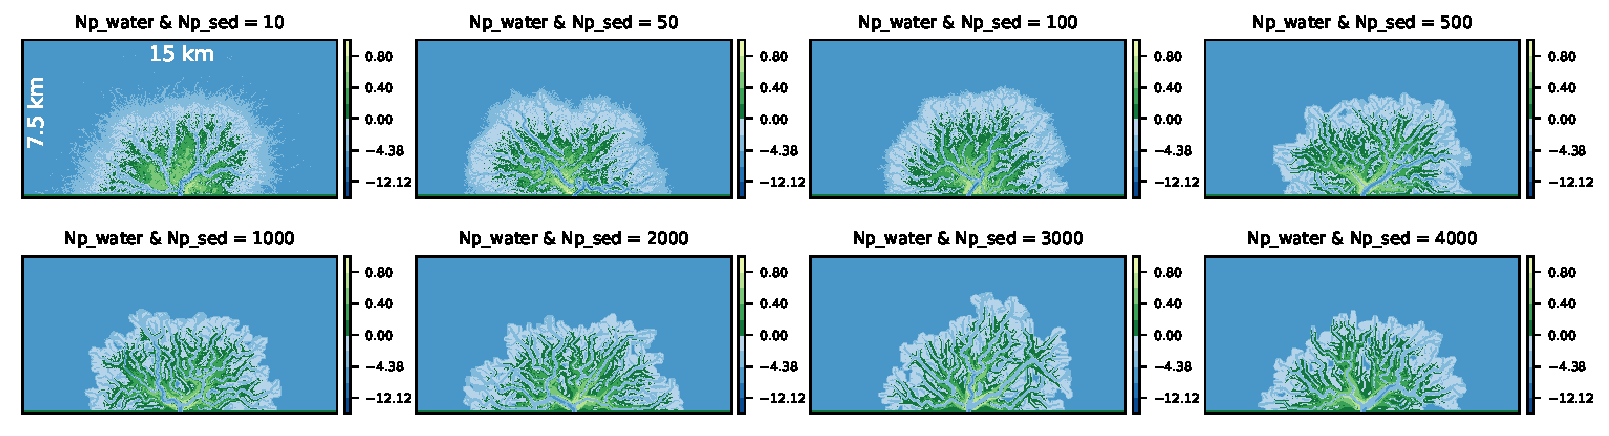
\includegraphics[width=\textwidth]{ParcelNumAnalysis/figs/full_varying_npboth.pdf}
	}	
	\caption{Final topographies when different numbers of parcels are used.}
	\label{fig:np_finaltopos}
\end{sidewaysfigure}

\begin{figure}[!ht]
	\makebox[\textwidth][c]{
	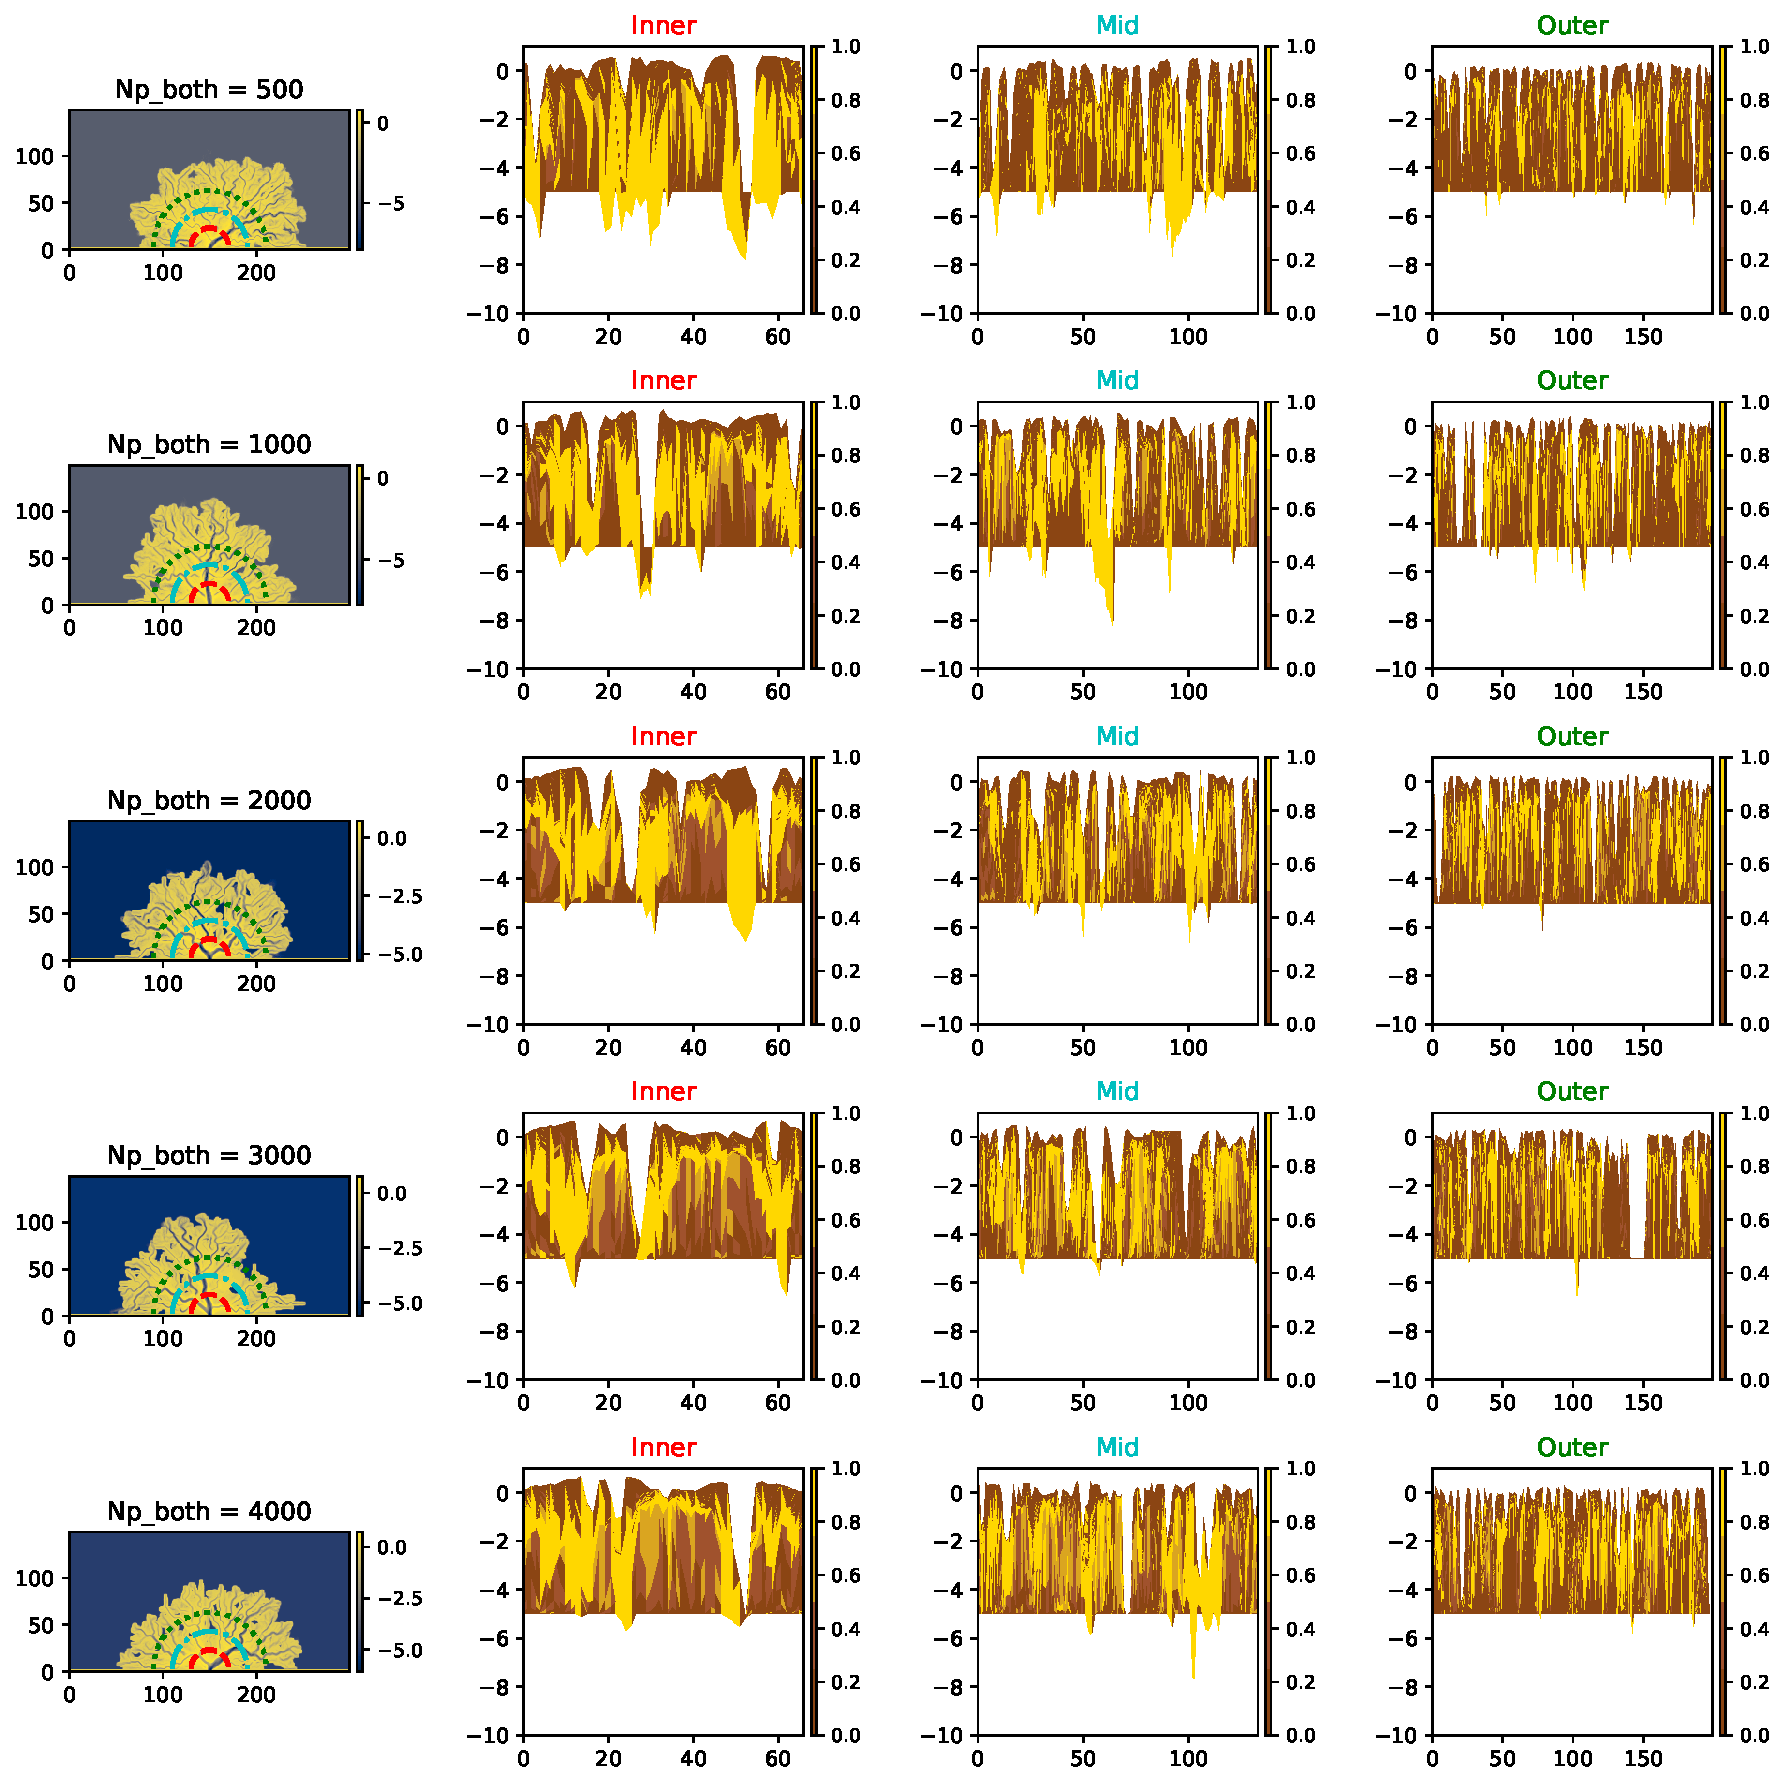
\includegraphics[width=\textwidth]{ParcelNumAnalysis/figs/npboth_sections.pdf}
	}	
	\caption{Sample topographic sections.}
	\label{fig:np_sections}
\end{figure}

\begin{figure}[!ht]
	\makebox[\textwidth][c]{
	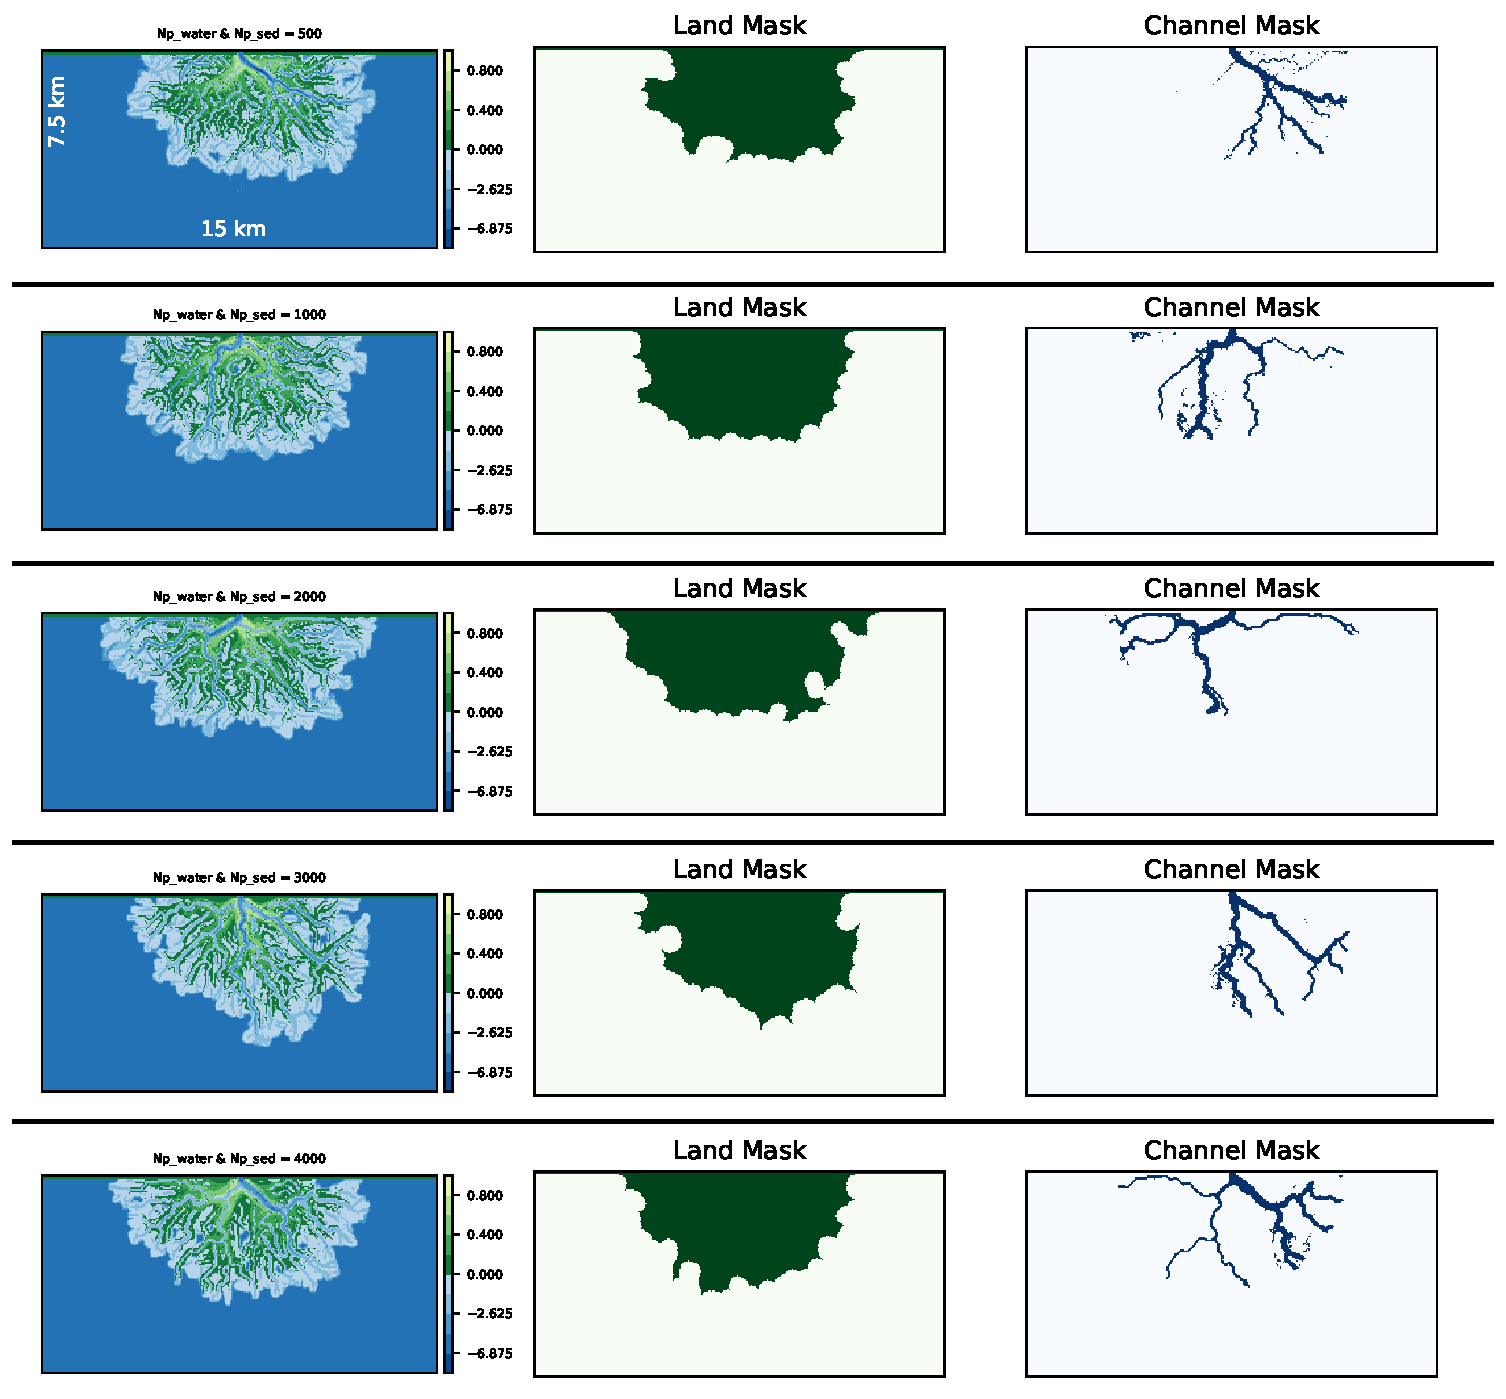
\includegraphics[width=\textwidth]{ParcelNumAnalysis/figs/varying_npboth_viz.pdf}
	}	
	\caption{Visuals of land masks and channel masks with their source topographies.}
	\label{fig:np_masks}
\end{figure}

\begin{sidewaysfigure}[!ht]
	\makebox[\textwidth][c]{
	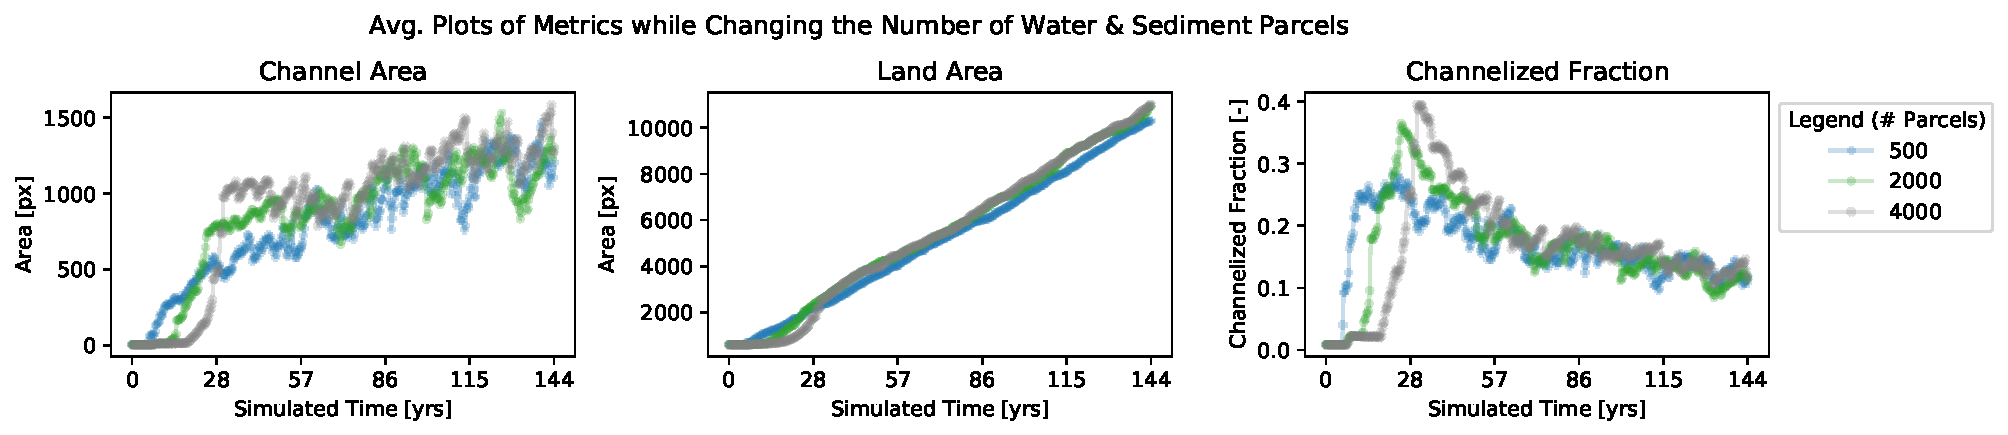
\includegraphics[width=\textwidth]{ParcelNumAnalysis/figs/npboth_avgmetrics_subset.pdf}
	}	
	\caption{Surface metric timeseries for three of the cases.}
	\label{fig:np_surfmetrics}
\end{sidewaysfigure}

\begin{figure}[!ht]
	\makebox[\textwidth][c]{
	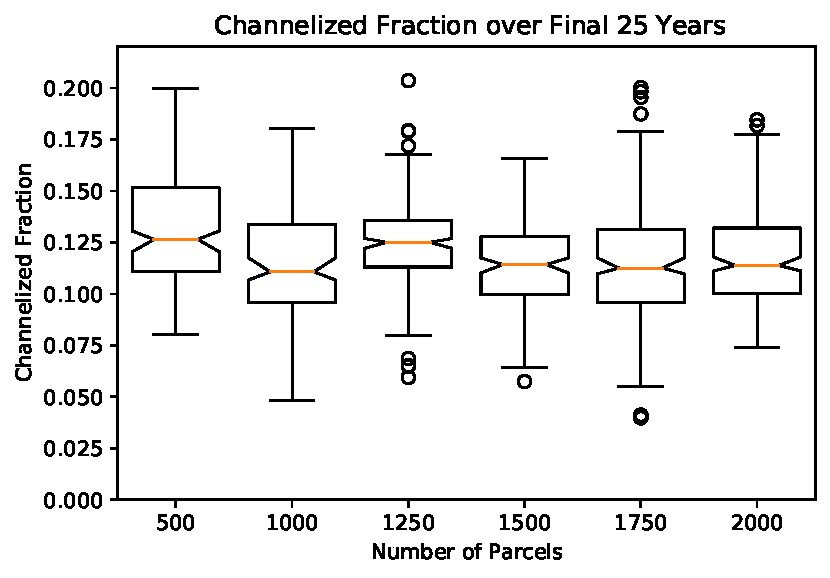
\includegraphics[width=\textwidth]{ParcelNumAnalysis/figs/midnp_cfrac_box.pdf}
	}	
	\caption{Box plots for the final 25 years split by parcel counts.}
	\label{fig:np_boxplots}
\end{figure}

\begin{figure}[!ht]
	\makebox[\textwidth][c]{
	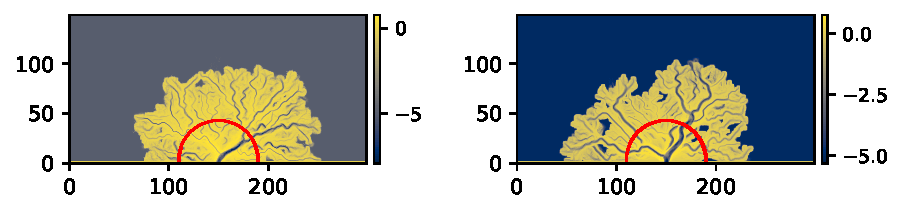
\includegraphics[width=\textwidth]{ParcelNumAnalysis/figs/midnp_sec.pdf}
	}	
	\caption{Visual of 2km azimuthal section locations.}
	\label{fig:np_radial}
\end{figure}

\begin{figure}[!ht]
	\makebox[\textwidth][c]{
	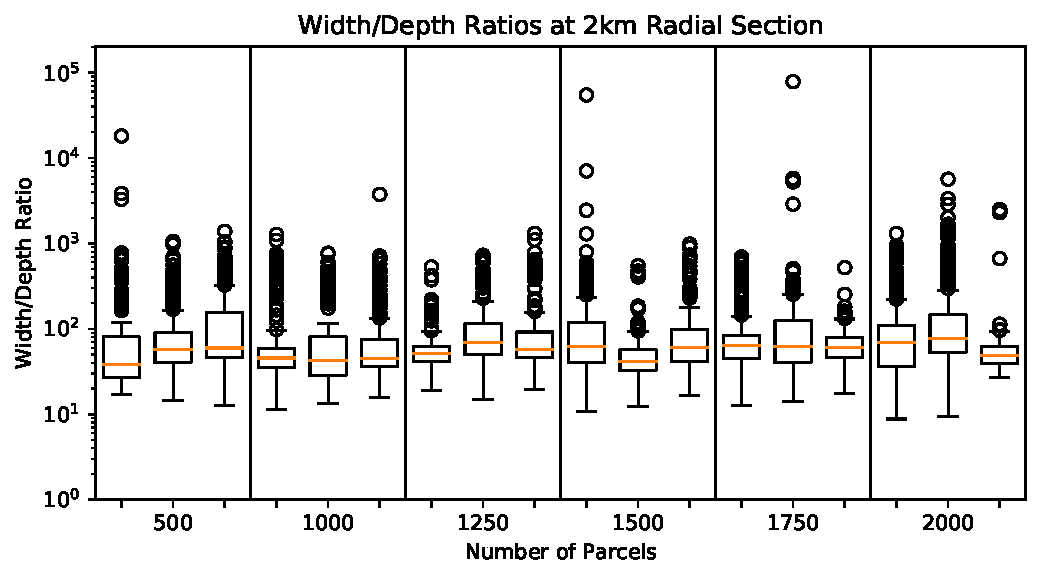
\includegraphics[width=\textwidth]{ParcelNumAnalysis/figs/midnp_widdep_box.pdf}
	}	
	\caption{Box plots of width-to-depth ratios for individual model runs grouped by parcel counts.}
	\label{fig:np_wd_box}
\end{figure}

\section{Conclusions}
Surprisingly, there are few obvious differences due to parcel numbers across the measured metrics.
When parcel numbers get really low (e.g., 50 parcels) it is clear that the model suffers; however once parcel counts get up to 500, especially once they reach 1,000 and greater, the models become very similar to each other.
This implies that we can push the model and get faster results by dropping parcel counts to 1,000 parcels rather than the 2,000 default value with little to no repercussions.

\clearpage
\bibliographystyle{plainnat}
\bibliography{bib/bib}